\documentclass[russian,utf8,landscape,a1paper,noignorestamp]{eskdgraph}
\usepackage[11pt]{moresize}
\usepackage{anyfontsize}

\ESKDdocName{\small{Разработка информационной системы автоматизация
удалённого мониторинга пациентов, нуждающихся в постоянном наблюдении на 
примере больных с ВПС}}
\ESKDscale{1:1}
\renewcommand{\ESKDcolumnXfIname}{Студент}
\ESKDauthor{Калесников Д.С.}
\renewcommand{\ESKDcolumnXfIIname}{Студент}
\renewcommand{\ESKDcolumnXfIIIname}{}
\ESKDchecker{Кошкин Н.Г.}
\renewcommand{\ESKDcolumnXfVname}{Руковод.}
\ESKDnormContr{Ванеев О.Н.}
\renewcommand{\ESKDcolumnXfVIname}{Зав. каф.}
\ESKDapprovedBy{Чичерин И.В}%  "Увт." в штампе на листе содержания
\ESKDdate{2013/05/18} % Дата (Год отображается на титульной странице)

\begin{document}
\ESKDstyle{formI}

\begin{figure}[h]
~\linebreak
\center{\fontsize{100}{110}\selectfont \bf Диаграмма классов}
~\linebreak
~\linebreak
~\linebreak
~\linebreak
\center{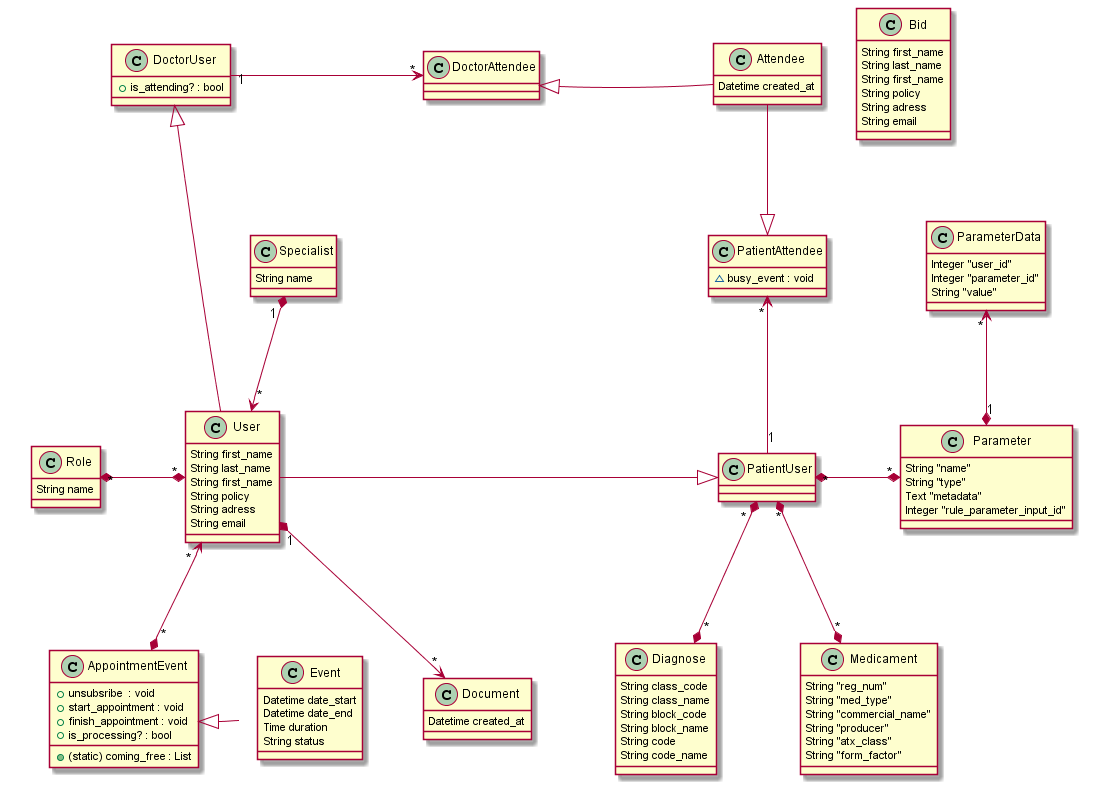
\includegraphics[width=0.7\linewidth]{../images/class_diagramm.eps}}
\end{figure}

\end{document}